\documentclass[spanish]{udpreport}
\usepackage[utf8]{inputenc}
\usepackage[spanish]{babel}
\usepackage{enumerate}
\usepackage[]{float}

\title{Ruteo Estatico y Dinamico}

\author{Javiera Araya,
       Benjamin Morales,
        Fabian Estefania,
        Nicolás Pino.\\
        Profesor:Jaime Álvarez.\\
        Ayudante:Maximiliano Vega.} 

\begin{document}
\maketitle




\chapter*{Resumen} 
\addcontentsline{toc}{section}{Resumen} 
\markboth{RESUMEN}{RESUMEN} 

El presente informe se basa en el funcionamiento del router para tener un conocimiento de la red en donde esta y el alcance de este, para ello se realizó una serie de actividades en donde se analizó de manera minuciosa como funciona cada router al momento de realizar las debidas configuraciones.  


\tableofcontents

\chapter{Introducción}

Para el correcto funcionamiento de una red es necesario que todos los routers que componen la red conozcan todas las distintas rutas que pueden alcanzar y cuales son viables para efectuar dicho trabajo, para ello es necesario interiorizarse sobre el funcionamiento del router y las estrategias que tiene que utilizar para realizar la toma de decisiones con respecto al camino o ruta más optima a utilizar. Las estrategias mencionadas anteriormente hacen referencia al ruteo estático y dinámico.

\chapter{Desarrollo}

\section{Actividad I: Topologia Base.}
Realizar la siguiente topologia en Packet Tracer.

\begin{figure}[H]
\begin{center}
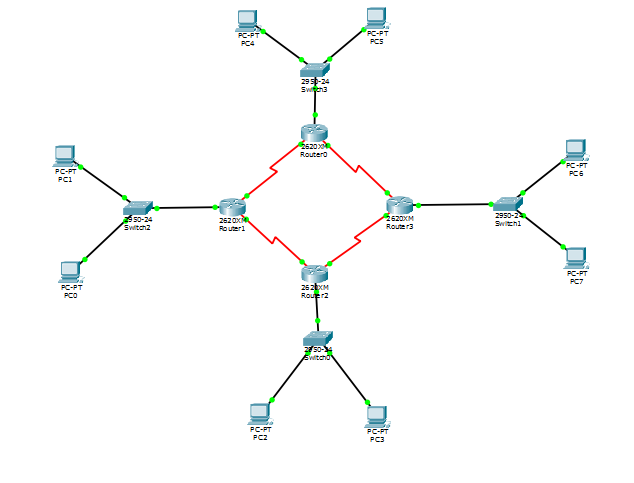
\includegraphics[scale=0.83]{images/Topologia.PNG}
\end{center}
\end{figure}
El primer paso fue incluir los routers "2620XM" y luego implementarles la interfaz "WIC-2T" a cada uno de ellos para asi poder conectarlos a travez de cable serial.

\vspace{16cm}



\section{Actividad II: Configuracion de Equipos.}

Conectamos los switches y PCs correspondientes dentro de la red para configurar cada una de las redes LAN en los routers.\\
\begin{figure}[H]
\begin{center}
Red LAN de Router0: 10.0.0.0/24\\
Red LAN de Router1: 10.0.1.0/24\\
Red LAN de Router2: 10.0.2.0/24\\
Red LAN de Router3: 10.0.3.0/24
\end{center}
\end{figure}
Todos los gateways de las redes LAN se definieron como "192.168.x.1", siendo "x" la red a la que pertenece la LAN. Como todas las redes LAN tienen prefijo 24, Todas las mascaras son "255.255.255.0".\\

Ejemplo:
\begin{figure}[H]
\begin{center}
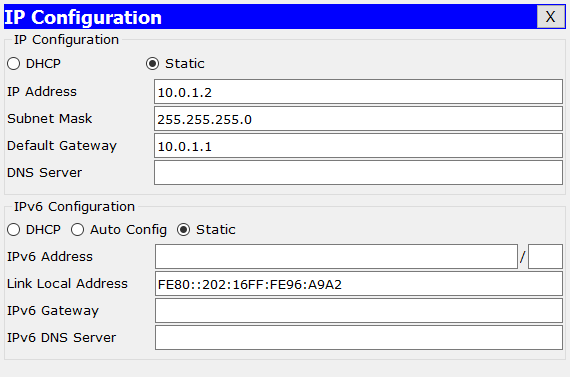
\includegraphics[scale=1]{images/ejemplo1.PNG}
\end{center}
\end{figure}

\vspace{16cm}
Luego se crearon redes para establecer conexiones entre los distintos routers implementados en la red.
\begin{figure}[H]
\begin{center}
Router0 - Router1 : 10.0.6.0/24\\
Router0 - Router3 : 10.0.7.0/24\\
Router1 - Router2 : 10.0.8.0/24\\
Router2 - Router3 : 10.0.9.0/24
\end{center}
\end{figure}

\begin{figure}[H]
\begin{center}
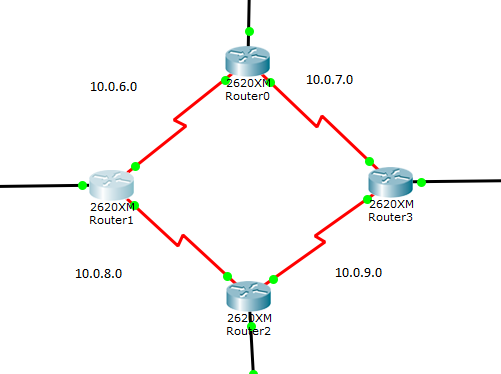
\includegraphics[scale=1]{images/Routers.PNG}
\end{center}
\end{figure}

\vspace{16cm}


\section{Actividad III: Configuracion de Ruteo Estatico.}

Para realizar esta actividad accedimos al terminal del router y utilizamos los siguientes comandos:\\

\begin{figure}[H]
\begin{center}
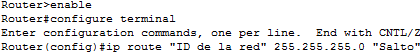
\includegraphics[scale=1]{images/comandos1.PNG}
\end{center}
\end{figure}

Donde ID de la red representa la red en la que quiero llegar y Salto representa la ip por la que debe seguir el paquete o mensaje. Por ejemplo si me encuentro en el Router0 y quiero llegar a la red 10.0.3.0 debo dar el salto al Router3 (10.0.7.2).\\

De esta manera se configuraron todos los routers implementados en la red asignadoles un camino estatico para cada una de las redes que no se encuentran a su alcance.\\

Ejemplo:
\begin{figure}[H]
\begin{center}
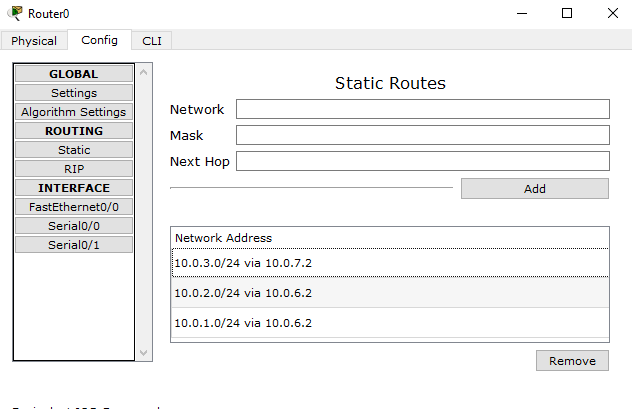
\includegraphics[scale=1]{images/static.PNG}
\end{center}
\end{figure}

\vspace{16cm}

\section{Actividad IV: Configuracion de Ruteo Dinamico.}

Para configurar el ruteo dinamico se sigue un proceso parecido al caso anterior solo que esta vez al router se le especifica que use ruteo dinamico y en que red se encuentra. Esto se realiza con los siguientes comandos:

\begin{figure}[H]
\begin{center}
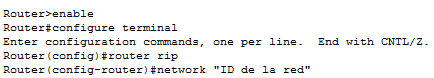
\includegraphics[scale=1]{images/comandos2.PNG}
\end{center}
\end{figure}

Donde ID de la red es la red que el router tiene conectado por LAN, por ejemplo para el Router0 el ID de la red seria 10.0.0.0, para el Router1 el ID de la red seria 10.0.1.0, asi sucesivamente.

\section{Preguntas}
\subsection{¿Qué ventajas y desventajas se pueden apreciar en cada tipo de enrutamiento?}

Una de las principales ventajas del enrutamiento estatico es el mayor control que se tiene sobre la red y poder dirigir los paquetes por donde sea mas comodo, gracias a esto se obtiene otra ventaja que es poder identificar mas rapido donde se producen los errores. La principal desventaja de este tipo de enrutamiento es la eficiencia ya que no se va a tomar la mejor ruta segun eficiencia, sino que solo tomara la ruta que se le asigno previamente, otro problema se da en el caso en el cual se caiga un enlace, la solucion a esto seria remplazar o reparar el enlace caido o asignarle una nueva ruta a los paquetes, en ambos casos se pierde eficiencia.\\

Una de las principales ventajas del enrutamiento dinamico a diferencia del estatico es la eficiencia, ya que los caminos se toman segun el numero de saltos que se deben dar, intentado dar el menor numero de saltos posibles, es mas facil y rapido implementarlo y ademas en caso de que se caiga un enlace el paquete tomara un nuevo camino sin necesidad de aplicar una nueva configuracion en la red, pero a causa de esto surge una de las desventajas en donde se pierde control sobre la red.\\

\subsection{¿En que se basa el enrutamiento dinámico para generar su ruta?}

La ruta por la cual se va el paquete en el enrutamiento dinamico depende del protocolo en que se base para generarla, estos protocolos se pueden dividir en 2 grandes grupos los cuales son:\\

Vector Distancia: Los protocolos basados en vector distancia para poder generar su ruta se basan en una metrica la cual depende de la cantidad de saltos que toma el paquete para llegar al destino y de esta forma elige la mejor ruta. Los protocolos vector distancia generalmente usan el algoritmo Bellman-Ford para la determinación del mejor camino.\\

Estado Enlace: Los protocolos basados en estado enlace para poder generar su ruta se basan en una metrica la cual genera un “mapa” de la red y mide el costo de llegar a cada uno de los routers vecinos, al terminar esto calcula la ruta de costo mínima al resto de los routers  con el fin de poder elegir la ruta que genere un costo menor. Los protocolos estado enlace generalmente usan el algoritmo Dijkstra para la determinación del mejor camino.\\

\chapter{Conclusión}

A partir de lo realizado en la presente experiencia de laboratorio, se logra destacar varios puntos, los cuales fueron fundamentales para el desarrollo de los objetivos propuestos, dichos puntos se especificaran a continuación.\\
Primero se armó una topología base, la cuál incluyó 4 routers conectados a través de cables seriales.
A cada uno de los router se les tubo que indicar a cuantas redes distintas podian acceder y por donde, para lo cual se utilizaron las estrategias de ruteo estático y dinámico.
Para ambos, se ingresó al terminal de cada router y se le ingresaron los comandos indicados en sus correspondientes actividades.\\
Probando las configuraciones en el software packet tracer, se logró comprender las ventenjas y desventajas de ambas estrategias, siendo estas escencialmente la eficiencia y el control sobre la red. 


\end{document}



